%!TEX root = ../main_text.tex

\chapter{Apêndices}


\begin{comment}
\section{\Benchmarks}
\citep{Trindade2016}

% intro
Por serem um excelente mensurador de performance de aplicações e processadores, \designs\ têm feito de \benchmarks\ uma parte crítica do processo de \design\ de projetos.
Uma vez que um \benchmark\ torna-se padrão e popular em um ramo de pesquisa, cria-se então uma alta pressão em aumento de performance por otimizações \citep{Hennessy2011}.

% utilização de benchs no trabalho
% arato2005
Para a demonstração e validação da solução a ser desenvolvida, será utilizado %vários \benchmarks\ e exemplos randômicos largos.
\benchmark\ de \textit{MiBench}.
Esse \benchmark, segundo \citeauthor{Guthaus2001} foi escolhido com base em um exame e comparação de um conjunto de aplicações embarcadas representativas comercialmente com o conjunto de \benchmarks\ SPEC2000 \citep{Case1995}.
\end{comment}


\begin{comment}
Por exemplo, considerando as vogais da língua inglesa onde o universo $ U = \{a, e, i, o, u, y\} $. 
Assim, uma partição desse problema $ \mathcal{X}_a $ de $ U $ pode ser representado por


\begin{equation}
\mathcal{X}_a = \left\{\{a, e, i, o, u\}, \{y\}\right\} \label{eq:xa}
\end{equation}

e supondo que o conjunto pode ser representando por cada unidade, uma outra forma de representação pode ser


\begin{eqnarray}
\mathcal{X}_b &=& \left\{\{a\}, \{e\}, \{i\}, \{o\}, \{u\}, \{y\}\right\}
\end{eqnarray}

Sobre tais conceitos, a Partição \ref{eq:part_c} viola a Equação \ref{eq:part_form_1} e a Partição \ref{eq:part_d} viola as Equações \ref{eq:part_form_2} e \ref{eq:part_form_3}.

\begin{eqnarray}
\mathcal{X}_c &=& \left\{\{a\}, \{e\}, \{i\}, \{o\} \right\} \label{eq:part_c} \\
\mathcal{X}_d &=& \left\{\{a, e, i\}, \{i, o, u, y\}, \{\}\right\} \label{eq:part_d}
\end{eqnarray}

A Figura \ref{fig:f4-2} ilustra o $ \mathcal{X}_a $ graficamente, segundo a Partição \ref{eq:xa}.

\begin{figure}[h] \centering
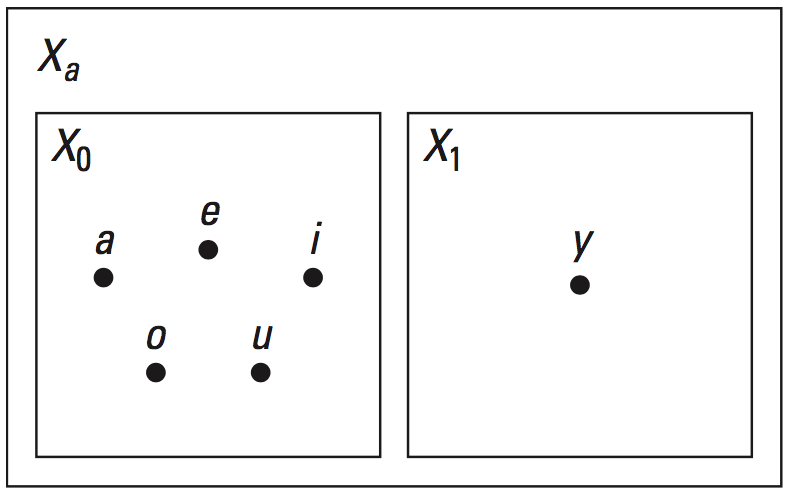
\includegraphics[width=0.5\textwidth]{img/f4-2.png}
\caption{Figura representativa do mapeamento da aplicação.}
\label{fig:f4-2}
\end{figure}
\end{comment}


%\chapter{Transferência de Estado} 

\section{Transferência de Estado} \label{chap:tranferencia}
   Segundo \citeauthor{Sass2010}, manter estado consistente sobre dispositivos FPGA e processadores é um desafio.
   Isso pois, como cada FPGA tem sua própria hierarquia de memória independente, estados são amplamente distribuídos no \design\ e há ampla variedade de interconexões entre FPGA e processadores.
   Assim, isso significa menos estados para serem transferidos e grande variedade de mecanismos disponíveis.
   Os tipos de estados serão descritos a seguir pois são requisitos para identificação de qual parte do estado da aplicação precisa ser explicitada pela comunicação processador e recurso.
   %Para entender melhor deve-se definir dois conceitos sendo eles estado afetado e preso ajudando a decidir quais partes do estado da aplicação necessitam de ser explicitamente comunicados entre processador e recurso.
   
   \begin{description}
      \item [Estado Afetado:]
      Na computação alguns estados são independentes pela construção e não precisam de ser transferidos de lugares. Retirando tais estados, restam os estados afetados.
      
      Esses, são os dados da aplicação que, durante a transferência de controle, podem ser modificados ou lidos por um recurso ou processador, necessitando de ser consistente entre todas as distribuições.
      %Estados afetados podem existir em grande escala. Principalmente quando arranjos, estruturas de dados complexas ou ponteiro estão envolvida e podem ser acessados de várias formas possíveis e geralmente não é possível saber se dois ponteiros estão apontando para um mesmo endereço.
      
      \item [Estado Preso:]
      Acontece quando parte da hierarquia de memória é compartilhada, nem todo o dado tem que ser explicitamente transferido e assim, caso todo o estado corrente esteja em memória primária (RAM) e ambos os dispositivos possuem acesso a ela, então não existe razão para a transferência explícita dos dados.
      
      Processadores modernos são construídos com quantidade significativa de memória que podem ser utilizadas como parte de estado sem a atualização da memória primária.
      Compiladores naturalmente utilizam toda a vantagem de registradores para armazenar os estados.
      
      Implementações em \hardware\ também incorporam dados ao longo do projeto e seus registradores e \textit{flip-flops} possuem valores intermediários entre ciclos de \textit{clock} dentro do projeto.
      O estado de uma aplicação é armazenado em várias partes do sistema.
      Para um recurso implementar parte de uma aplicação, precisa-se então integrar-se com parte do estado.
      
      Esse pode ser considerado mais facilitado pelo fato de que o estado está localizado em um espaço comum. Mas se um estado está localizado num registrador ou em uma cache de um processador, ele não pode ser acessado pelo sistema externo e, neste caso, o estado encontra-se preso e deve ser explicitamente transmitido pela interface.
      
      \begin{figure}[h] \centering
         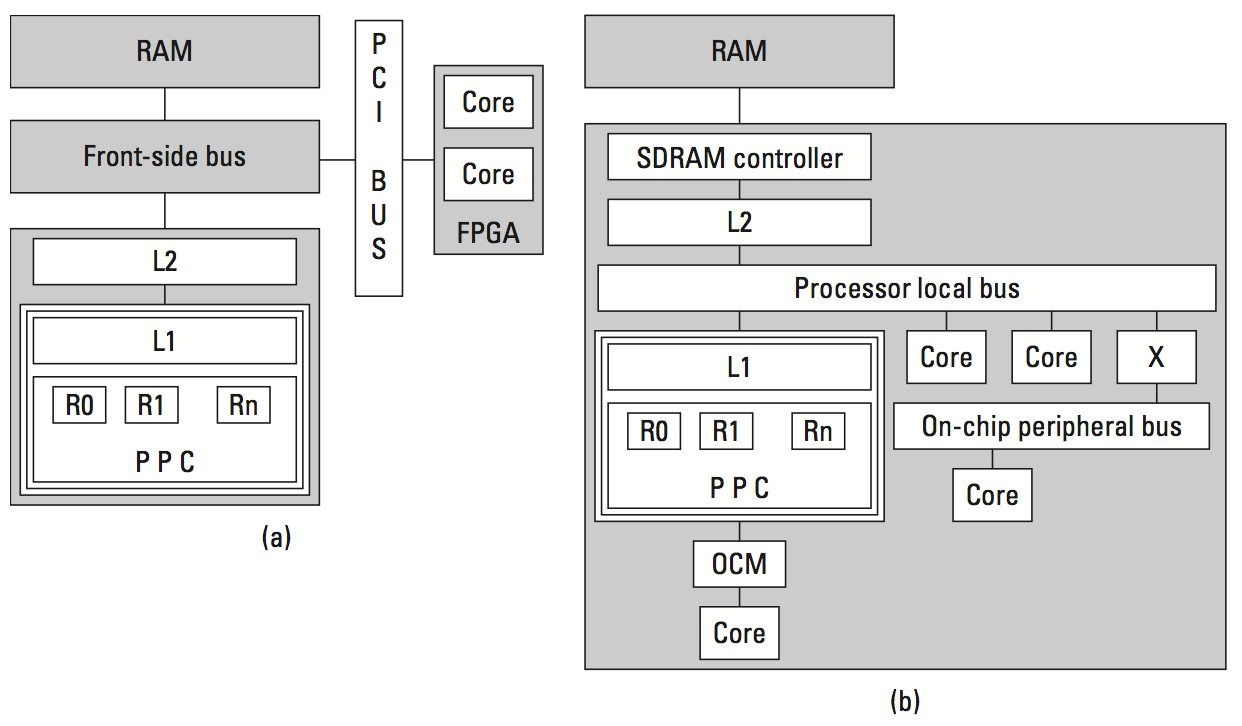
\includegraphics[width=1\textwidth]{img/f4-7.png}
         \caption{Situações na qual pode ocorrer bloqueio de estado. \textit{a)} Situação na qual existe um processador externo ao FPGA e sua memória interna é inacessível. \textit{b)} Situação onde o processador situa-se na plataforma FPGA. Fonte: \citet{Sass2010}.}
         \label{fig:4-7}
      \end{figure}
      
      Em ambos os casos mostrados na Figura \ref{fig:4-7} o FPGA (representado pelos \cores\ não possui autorização para o acesso aos registradores do processador (representados por $R_n$). Mesmo em \textit{b)} onde o processador é integrado à plataforma FPGA, não possui-se acesso sendo necessário a disponibilização manual deste.
   \end{description}
   
   
   \section{Problema de Transferência de Estado}
   Estados afetados que estão presos necessitam de ser explicitamente comunicados e esta é feita por um processo chamado \textit{marshaling}.
   Assim, será feito um \textit{Marshaling} de grupos de elementos de um estado afetado de uma aplicação em registros lógicos que são explicitamente transferidos.
   
   Tendo a premissa que o processador possui o controle inicial, tem-se quatro tipos de registros que podem ser utilizados.
   Os dois primeiros, \textit{Type-I} e \textit{Type-F}, são utilizados para iniciar e outro para finalizar a transferência de um conjunto de elementos para o recurso, respectivamente.
   Os outros dois tipos de \textit{marshal} são usados repetidamente. Um quando o recurso é invocado (\textit{Type-CI}, do inglês \textit{copy-in}), e quando é completado (\textit{Type-CO}, do inglês \textit{copy-out}).
   %Um exemplo de \textit{Type-F} é quando tem-se um \core\ que acumula um valor em uma variável global. O registro \textit{Type-F} seria utilizado para ler o valor da variável após sua última invocação.
   
   Um processo de tradução pode ser incorporado com o \textit{marshaling}, sendo o exemplo a conversão de ponto flutuante para fixo quando transferido para um recurso o que acontece também com transformações mais complexas.
   %O agrupamento de elementos é lógico pelo fato do \textit{assembly} não significar estritamente que os elementos são copiados para uma memória de locação contínua.
   
   A forma mais simples de transferir estados é copiando os registros, parando o processador enquanto o recuso processa.
   Este é chamado de \textit{push} os dados no qual transmite o dado antes da transferência do controle. Ao final, realiza-se o \textit{pulls} dos dados.
   
   
   Embora isso, uma transferência instantânea de estado não é sempre simples. Quando o estado afetado é grande mas o dado atua é pequeno, o padrão de acesso ao dado é randômico e a transferência lógica de registro é larga sendo mais vantajoso o uso de interfaces de comunicação para servir o recurso. Ou seja, utilizado quando o recurso foi designado para reduzir a latência da tarefa e a transferência do registo é pequena.
   Quando o registro lógico e o dado atual são largos, utiliza-se de padrão de acesso regula que transmite dados continuamente. É usado quando o recurso aumenta o \textit{throughput} e a redução de latência ou metas de performance não são possíveis.
   
   Isso é útil por exemplo na ordenação onde transferir um arranjo completo quando invocado é uma operação cara e desnecessária já que dependendo do algoritmo, pode-se utilizar apenas frações deste.



\section{Análise de Performance de Sistema} \label{sec:amdahl}
	A análise de performance de um sistema é definida pela Lei de \citeauthor{amdahl1967validity} de \citeyear{amdahl1967validity} relaciona o tempo gasto para executar uma tarefa com um único processador e o gasto com $j$ processadores. Nessa definição, $T_1$ representa um computador sequencial e $T_j$ um computador com $j$ núcleos. Sendo $s$ a fração relativa ao trecho estritamente serial e $q$ a fração relativa ao tempo paralelizável, tem-se as seguintes definições básicas

	\begin{eqnarray}
		T_1   & = & s + q = 1\\
		T_j & = & T_1 \times s + T_1 \times  \left(\frac{q}{j}\right)
	\end{eqnarray}

    O \textit{speedup}, cálculo do ganho da utilização de vários \cores, é obtido pela Fórmula \ref{eq:spu_init}.

	\begin{eqnarray}
		Speedup & = & \frac{T_1}{T_j} \label{eq:spu_init}
	\end{eqnarray}

	Dessa forma, realizando substituições das definições básicas na Equação \ref{eq:spu_init}, tem-se a Equação final de \speedup\ em \ref{eq:spu_fim}.

	\begin{eqnarray}
		Speedup & = & \frac{T_1}{T_j} = \frac{(s + q)}{\left(s+\frac{q}{j}\right)} = \frac{1}{\left(s+\frac{q}{j}\right)} \\
		%T(n) & = & T(1)(B + \frac{1}{n}(1 - B)) \\
		Speedup & = & \frac{1}{s + \left(\frac{1 - s}{j}\right)} \label{eq:spu_fim}
	\end{eqnarray}

	Essa equação articula os limites de um melhoramento global para uma aplicação que um simples aprimoramento pode fazer em tempo de execução.

	Generalizando a equação para incluir todo potencial de aprimoramento e métricas de performance arbitrária, pode-se caracterizar os limites como coleções de aprimoramento.
    Se esses aprimoramentos são recursos de \hardware\ e podemos antecipar o ganho requerido ganho potencial de recursos para cada recurso, então pode-se desenvolver um modelo que irá orientar ao processo de particionamento.

    Tal lei não é adequada pois:
	\begin{itemize}
		\item Visa um simples realce e não nos auxilia a selecionar um subconjunto de uma coleção de recursos potenciais;
		\item Foca somente no tempo de execução;
		\item Não visa recursos requeridos;
		\item Não visa custo de comunicações.
	\end{itemize}

	Perfis baseados em exemplos requerem representações de entrada e é uma aproximação de tempo gasto. Sem implementar todo o potencial de recursos em \hardware, pode ser difícil antecipar os recursos requeridos. Pode-se com determinação analítica calcular quantos ciclos de \textit{clock} um recurso de \hardware\ irá tomar, podendo assim calcular métricas como \speedup. Entretanto, é impossível saber quando um processo arbitrário será completado. Ao invés de prover uma solução automatizada, a solução analítica simplesmente provê um \textit{framework} para guiar um \designer\ de sistema a criar uma solução criativa.

	\subsection{Abstração e Estado}
		No contexto de desenvolvimento, um módulo é uma abstração de alguma funcionalidade em um sistema.
		A palavra abstração é definida como `operação intelectual em que um objeto de reflexão é isolado de fatores que comumente lhe estão relacionados na realidade', ou seja, no sentido amplo da palavra, significa tirar fora, extrair, remover.
		Um módulo tenha uma boa abstração terá suas interfaces e descrições mais fáceis de serem compreendidas, entretanto isso torna sua implementação mais complexa.
		Uma boa abstração capta todas características importantes de algo criando assim uma organização e dessa forma, uma representação rica em informação pode não ser tão relevante\todo{rever}.
		Em contra partida, caso seja feito uma abstração ruim de algo, forçará-nos a pensar não só sobre a singularidade do módulo, mas também como foi implementado, o que não é uma informação valiosa para uma abstração.

		Estado é uma palavra já conhecida no âmbito de sistemas eletrônicos. Estados são explicitados num \design\ de máquinas sequenciais por exemplo, e podem ser um ponto de memória de dispositivos eletrônicos.
		Em sistemas embarcados, sua definição é um pouco mais abstrata à dita já que um estado de módulo pode ser armazenado em vários lugares em várias formas distintas como \textit{flip-flops}, \textit{static RAM}, arquivos, ou até mesmo em memórias \textit{off-chip}. Dessa forma, estado pode ser definido como uma condição de memória onde é possível segurar uma informação por um certo período de tempo.

	\subsection{Coesão e Acoplamento}
		Definido o conceito de abstração e estado de sub-rotinas, é necessário esclarecer os conceitos de mensurações sobre módulos sendo essas coesão e acoplamento.

		Coesão é uma métrica de abstração. Assim, se os detalhes dentro de um módulo no ato da implementação são funcionalidades compreendidas facilmente, então o módulo possui coesão.
		O acoplamento é a forma de como os módulos estão relacionados uns com os outros. Uma dependência entre módulos existe quando um comunica diretamente com outro. Quando um módulo \A\ invoca um módulo \B, então \A\ depende de \B. Entretanto, \B\ não necessariamente depende de \A.

		Dependências não são sempre explícitas e com isso entra-se o conceito de estado para auxiliar na formação de um módulo.
		Quando dois módulos parecem não ter nenhuma dependência entre si mas o sistema exige que ambos tenham terminado seus processamentos ao mesmo tempo, cria-se então uma dependência e etiquetados como dependentes por temporização. O fato de dois módulos serem utilizados no mesmo estado os tornam dependentes.

		São necessárias para que o procedimento possa funcionar corretamente com todos os outros módulos, mas precisa-se saber o grau de acoplamento em número e tipo.
		%Dependência surgidas a partir de interfaces formais possuem  são as melhores formas de dependências.
		Uma forma de reduzir acoplamento em sistemas são por meio de encapsulamentos. Eles envolvem manipulações de estado e introdução à interface formal sendo a ideia principal a movimentação de um estado dentro de um módulo e fazer com que isso seja exclusivo, ou seja, não compartilhado, técnica bastante eficaz. Pode ser reconhecida também como informação escondida.
		Ao realizar tal procedimento, permite-se maior liberdade de mudança interna no módulo pois, alterando seu estado, a mudança deste não introduz erro em outro módulo consequente. E se o módulo possuir uma boa abstração, então a informação escondida também permite que o módulo seja implementado de forma mais independente.

		É preciso evitar acoplamentos quando desnecessário e para isso existem várias técnicas para manipulação do grau de acoplamento. Uma fácil de ser resolvida é como exibida na Figura \ref{fig:acoplamento}. Em a) que os sub-módulos \B\ e \C\ possuem dependência do módulo somatório \A. Na Figura \ref{fig:acoplamento} b) o somatório \A\ é duplicado dentro de cada sub-módulo eliminando cada uma das dependências existentes, reduzindo o fator de acoplamento.

		\begin{figure}[h] \centering
			\includegraphics[width=0.6\textwidth]{img/f3-4.png}
			\caption{Exemplo de redução do fator acoplamento em um módulo.}
			\label{fig:acoplamento}
		\end{figure}

		%Será proposta uma situação exibindo o porquê desta abordagem pode ter mais vantagens: suponha que A foi designado para calcular somente números não-sinalizados. Mas com o passar do tempo, C necessita de operar com número sinalizados. Dessa forma, na Figura \todo{a} o \design\ deveria alterar tanto C quanto A. Alterando A, obrigatoriamente afetará B. Mesmo que B continue a trabalhar bem com a alteração de A, ouve uma cascata de alterações a serem feitas ao longo do tempo sobre algo que deveria ser pequeno, simples e isolado.

		%Discutindo sobre desvantagens deste procedimento, talvez se pensa que isso pode aumentar no tamanho do \design\ do projeto já que está duplicando um item, mas não. É possível que a funcionalidade de A seja simplesmente mesclado com o configurable logic block (CLB) já alocado para os sub-módulos B e C e consequentemente é possível que não haja nenhum ganho de conexão no CLB alocado. É claro que isso não é sempre verdade e é possível sim que tenha aumento de custo. Uma segunda desvantagem é, ao duplicar um módulo, agora se tem o mesmo componente em dois lugares. Se um erro for encontrado em um, deverá ser alterado noutro também.



\subsection{Invocação e Coordenação}

	Da mesma forma que modelos de computação sequencial e \textit{multithread} podem realizar invocações de sub-rotinas, o mesmo pode ser realizado em \hardware\ com o codinome de política de coordenação. Em nível de \hardware\ existe diferenciações pois neste não existe controle de de \textit{thread} mas geralmente possui somente um controlador que habilita ou não o recurso para processamento. Muitas máquinas de estado têm uma ordem de estados \textit{idle} e a transferência de controle pode ser a sua ativação. Existe três abordagens para coordenar um \hardware\ e \textit{\software} e serão descritas a seguir.


	\subsubsection{Modelo de Coprocessador}

		Também conhecido como modelo \textit{go/done} ou modelo cliente/servidor, o modelo coprocessado é similar a sub-rotina chamada acoplamento. Neste modelo, o \hardware\ fica em estado neutro, esperando fornecer um serviço para o processador. O processador envia um sinal de início e espera o resultado. Neste modelo, todo recurso em \hardware\ deve ter o estado \textit{idle} já definido em \design\ e padronizado para iniciar em modo desligado. Um item importante nesse sistema é saber manusear o tempo enquanto o recurso está operando algumas formas em especiais serão citadas a seguir.


		\paragraph{Fixando o Tempo}

			Para recursos de pequeno porte que possuem um tempo fixo, o mecanismo mais eficiente é o processador realizar um número de instruções ``\textit{no-op}'' para que em seguida possa receber o resultado sempre checando o sinal \textit{done}.



		\paragraph{\textit{Spin-Lock}}

			Quando o total de tempo é desconhecido, utiliza-se mecanismo de \textit{spin-lock}. É um processo conhecido como \textit{pooling} onde o processador fica num processo repetitivo de questionamento ao recurso se sua operação já foi finalizada.



			\begin{verbatim}
				// Simple y = m*x + b Example
				invoke_hw(m, x, b);
				while(!done) {
				    done = check_done_signal();
				}
				y = retrieve_results();
			\end{verbatim}



		\paragraph{Bloqueio}

			A forma tradicional utilizada nesta situação é tratar o recurso como um dispositivo de I/O. O sinal \textit{done} pode ser tratado como uma interrupção ao processador no qual permite o recolhimento do resultado.

			\begin{verbatim}
				// Simple y = m*x + b Example
				invoke_hw(m, x, b);
				yield();
				y = retrieve_results();
			\end{verbatim}



		\paragraph{Solução Especial para o Modelo de Coprocessador}

			A transferência de um estado de \hardware\ para \software\ é muito das vezes impraticável. Determinando primeiramente os métodos, o algoritmo foca nos locais mais prováveis para a extração de recursos.

			Um grafo de chamadas estático é construído e a recursão é utilizada para detectar componentes fortemente conectados do grafo e retirados de consideração.

			\begin{figure}[b] \centering
				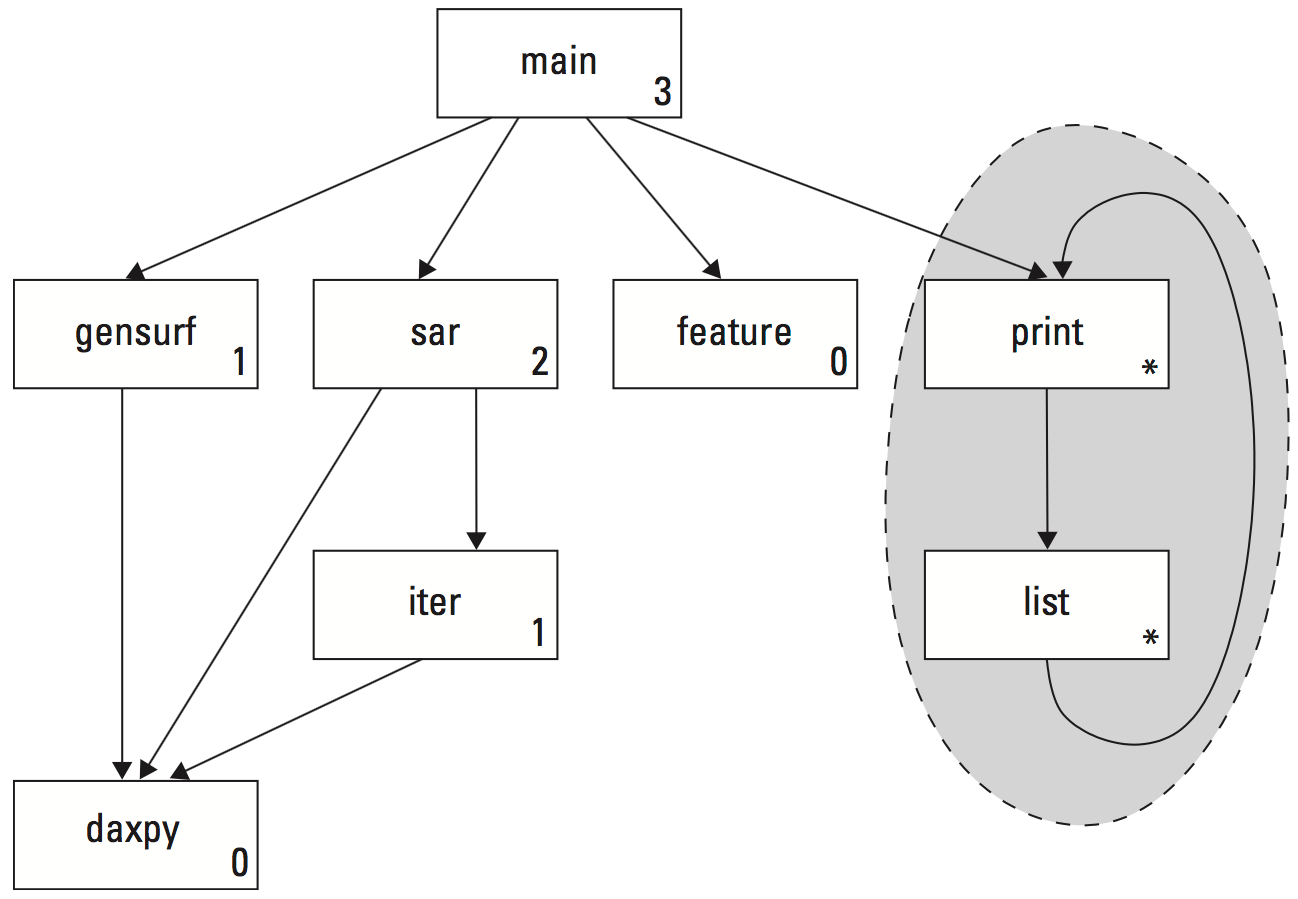
\includegraphics[width=0.6\textwidth]{img/f4-4.png}
				\caption{Análise de funções na qual os comandos \texttt{print} e \texttt{list} repetem inúmeras vezes.}
				\label{fig:perf_print_list}
			\end{figure}

			O exemplo da Figura \ref{fig:perf_print_list} mostra que as funções \texttt{print} e \texttt{list} formam um componente fortemente conectado e são marcados com um *. Em seguida, os vértices restantes de $ G $ são assinalados por uma regra ordinal,

			$$
			\text{ord}(u) =
			\left\{\begin{matrix}
			0 & \text{se nó } u \text{ é uma folha} \\
			\underset{(u,v) \in E(G)}{\max}\ \{ \text{ord}(v) \} + 1 & \text{caso contrário}
			\end{matrix}\right.
			$$


	\subsubsection{Modelo \textit{Multithread}}
		Além do modelo coprocessado, tem-se o modelo \textit{multithreads} que emerge como uma importante técnica de programação utilizada até em computadores com multiprocessadores. Neste modelo, o paralelismo natural do \hardware\ é conhecido e o \designer\ reconhece que o processador e os componentes executam continuamente. A coordenação desses componentes é manuseada por comunicações primitivas que tem sido desenvolvidas por processo concorrentes como semáforos, mensagens e outros. Cada \hardware\ é considerado um componente que executa como uma \textit{thread} paralela e o sistema de semáforos é utilizado para deixar o sistema consistente e assim, ao invés de bloqueado, o \hardware\ conceitualmente fica em bloqueio esperado pelo semáforo ou por uma mensagem.


	\subsubsection{Modelo de Rede em Chip}
		Este modelo investiga o estado distribuído completamente e depende da troca de mensagem para explicitar o estado. A coordenação é implícita com a transferência de estado. Como é assumido que o \design\ referencial de \software\ foi construído com comandos de troca de mensagem explícita, não se considera em um manual de sistemas embarcados. Entretanto, tem-se visto que técnicas de alta-performance continuam filtrando-se para o nível de sistemas embutidos.


\section{Programação Linear Inteira (PLI)} \label{sec:pli}
	Este problema representa um subgrupo da programação linear no qual algumas ou todas as variáveis do problema pertencem ao conjunto dos números inteiros. A tentativa de solucionar um PLI para um modelo puro com quantidades de restrições é um problema $\mathcal{NP}$-difícil.

	Um modelo de PLI pode ser obtido com a seguinte característica:

	\begin{equation}
			\begin{array}{rrcll}
			\text{min}  &  c' x    &  ~     &  ~            &  ~               \\
			subject\ to &  a'_i x  &  \leq  &  b_i,         &  \quad i \in M_1 \\
			~           &  a'_i x  &  \geq  &  b_i,         &  \quad i \in M_2 \\
			~           &  a'_i x  &   =    &  b_i,         &  \quad i \in M_3 \\
			~           &  x_j     &  \in   &  \mathbb{Z},  &  \quad j \in N_1 \\
			~           &  x_j     &  \in   &  \mathbb{Z},  &  \quad j \in N_1 \\
			\end{array}
            \label{eq:constraints_pli}
	\end{equation}
    
    onde:
    
    \begin{description}
    	\item [$c'x:$] é uma função linear de custo;
    	\item [$x:$] variáveis de decisão;
    	\item [$a':$] coeficientes fixos;
    	\item [$a'x \leq b, a'x = b$ e $a'x \geq b:$] restrições para validação da solução.
    \end{description}


\section{Questões} 

	\subsection{\textit{Profiling}} \label{sec:dificuldades}

			Uma suposição não adequada com a formulação analítica é que ela usa informação de \textit{profile} para aproximar o tempo de fração que uma aplicação gasta em uma sub-rotina ou bloco básico, mas no entanto, várias situações podem gerar resultados enganosos.



		\subsubsection{Execução Dependente de Dados}

			Quanto um simples conjunto de dados não representa o tempo gasto de cada sub-rotina quando este é alterado a sub-rotina não terá mudanças substanciais com a mudança do dado de entrada. A detecção da situação onde um único conjunto de dados não é representativo torna a situação difícil e requer que o \designer\ do sistema compreenda a operação fundamental da aplicação como é o caso da análise de complexidade das rotinas. É possível analisar esses casos com alguns métodos sendo a análise manual dos algoritmos e suas operações básicas, a coleta de informações \textit{profiling} baseado em diferentes conjuntos de dados ou mesmo a tentativa de separar a aplicação talvez ao longo dos limites do módulo e fazer o \textit{profile} de cada módulo independente.

		\subsubsection{Comportamento Correlacionado}

			Outra questão surge em aplicações que explicita o uso de eventos cronometrados. Muitos \textit{profile} assumem que a aplicação fará um progresso estável em direção à solução mas algumas aplicações incorporam o tempo. Sistemas de \textit{profiles} usam um temporizador de intervalo para amostrar o contador de programas dependendo da aplicação para não serem correlacionados estatisticamente com o temporizador. No entanto, se a aplicação possui operações executando em tempos regulares, periódicos, então os resultados do \textit{profiling} podem ser considerado enganosos. Por exemplo, se uma aplicação é executada a cada 10ms e a amostragem é feita a cada 10ms, então o \textit{profiler} não fornecerá dados concretos referentes ao sistema.



		\subsubsection{Comportamento Faseado}

			Sobre a totalidade de sua execução, o controle se move entre \textit{clusters} de operações relacionadas, isso é, a execução de uma aplicação exibida localmente. Como um exemplo, consideremos uma aplicação que possui três rotinas. Assumindo que cada possui $ 33\% $ de tempo de execução, e que cada tem a possibilidade de ter um \speedup\ de 50\% e postas de forma ordenada da primeira à última. Se existe espaço somente para uma rotina em recursos de FPGA, então o \speedup\ máximo será de 12\%. Mas se o comportamento faseado é suportado pelo \design\ de sistema, então há mais opções. Um é olhar procurar itens em comum sobre os três \textit{cores} e uma segunda é um \hardware\ multiplexado por tempo. Não há abordagens automáticas para esse.



		\subsubsection{Efeitos de I/O}

			\textit{Profiles} não contam tempo de I/O tais como acesso ao espaço de usuário e dispositivos realizando algum procedimento de busca ou ação.



		\subsubsection{Números de Chamada}

			\textit{Profiles} entretanto continuará a calcular quando sub-rotinas são invocadas. É importante ter noção o quanto uma sub-rotina é invocada.

	\subsection{Estrutura de Dados}

		Design de referência de \software\ naturalmente reflete um viés em relação às implementações em \software. Isso é compreensível, já que a programação é ensinada no contexto de modelo de computação sequencial ordinário. Com esses modelos, a diferença entre

	\begin{verbatim}
	while( i!=NULL ) {
	  proc(i) ;
	  i = i->next ;
	}
	\end{verbatim}
	e
	\begin{verbatim}
	while( i<n ) {
	 proc(x[i]) ;
	 i=i+1;
	}
	\end{verbatim}

		é insignificante já que ambos tomam $ \mathcal{O}(n) $ passos, mas em nível de \hardware\ o último pode ser mais desejável sendo no mínimo, uma ampla janela de pré-busca é possível. Se pudermos determinar que, em várias iterações do ciclo, cada \texttt{proc(x[i])} é independente, então pode-se melhorar o \design\ por meio de \textit{pipeline} ou paralelismo regular.

		O \design\ de referência de \software\ serve como extremamente bem como uma especificação, mas se executar um \textit{profile} do \design\ de referência, não será capturado os benefícios da implementação pois esses benefícios provem de alterações algorítmicas e são improváveis de serem reveladas por técnicas automáticas. Consequentemente, cai sobre o \designer\ de sistema compreender ambos o algoritmo de \software\ implementado no \design\ referencial e como pode ser re-implementado em \hardware.

		Há vários formas comuns de estruturas de \software\ que pode ser rearranjadas para produzir melhor \design\ de \hardware. Estruturas de dados que utilizam ponteiro como listas encadeadas, árvores, etc. podem ser representadas por uma estrutura ``\textit{flat}'' como vetores e arranjos produzindo acesso regular em memória que podem ser pré-buscadas subsequentemente ou utilizadas em \textit{pipeline}. Outra forma de ganho de performance é no tamanho de bit. Programadores de \software\ geralmente assumem um valor fixo, mesmo que utilizem somente poucos bits de informação. Enquanto \software\ tem caminho de dados fixos e relativamente baixa largura de banda entre componentes, \hardware\ se destaca no gerenciamento de largura de bits arbitrárias sendo possível alavancar grande largura de banda fornecida pela interconexão programável do FPGA.

	\subsection{Manipulando Tamanho de Recurso}

		A mudança mais simples envolve quebrar uma sub-rotina em sub-rotinas menores fazendo com que o recurso em \hardware\ fique menor e mais fácil de ser implementado.

		Há três momentos que agregar sub-rotinas são necessárias. Se duas sub-rotinas tomam 25\% cada uma do tempo da aplicação, então elas são candidatos fortes para a implementação em \hardware. No entanto, se for implementado individualmente, cada uma invoca o custo da sua interfaceação. Se há três sub-rotinas relacionadas (uma invocando a próxima), então a combinação delas pode reduzir o custo de invocações. Entretanto, o custo da interface não é sempre insignificante e vale a pena o esforço do usuário para investigar a situação.

		Qualquer outra mudança é substancial. Frequentemente, implementação em \hardware\ tem performance significativa por ter formato de dados de dados específicos da aplicação. Para que o \software\ seja mais eficiente nos formato de dados não padronizados, programadores irão investir em estruturas de dados que não são bem mapeadas para o \hardware. Assim, vale a pena olhar para o propósito e considerar a substituição de estruturas de dados para melhor explorar o \hardware.





\begin{comment} %comment Módulos e Interfaces em \Design\ de \Software
\section{Conceitos e Componentes de \Design\ de Sistemas}
% \subsection{Módulos e Interfaces}
%Existem duas filosofias de \design\ para a construção de um sistema. Em um delas é possível realizar a especificação de cada função do projeto, chamado de blocos básicos\footnote{Um bloco básico é uma sequência maximal de instruções sequenciais com \textit{single entry and single exit} (SESE).}, e conectá-los logicamente de acordo a fim gerar o sistema completo. Tal é descrito como abordagem \textit{bottom-up}.
%A segunda baseia-se na descrição de um sistema completo e geral sendo que, em seguida, o \designer\ desmembra-o definindo seus sub-blocos até chegar ao nível mais básico de suas funções. Essa é chamada de abordagem \textit{top-down}.
%O conceito de abordagem de desenvolvimento de projetos é importante para descrever os conceitos de módulo e interface.%, segundo \citet{Sass2010}.

\subsection{Módulos e Interfaces em \Design\ de \Software}
\citet{Sass2010}, em seu livro, descreve que módulo é qualquer conjunto de operação auto-contidas que possui um nome, interface formal e geral e alguma descrição funcional. Isso significa que qualquer procedimento, mesmo que em \software\ ou em descrição de \hardware, que possa ser representado por uma caixa graficamente é considerado um módulo.
Define-se por interface formal o nome do módulo e a enumeração de duas operações, incluindo suas entradas e saídas, caso existam e a interface geral inclui todas as características da interface formal e qualquer protocolo ou comunicação adicional implícita. Com a interface formal descrita, é possível realizar inspeções mecânica e técnica no módulo enquanto a geral, o entendimento desse em alto nível.
Por último, um módulo pode ter também uma descrição funcional no qual pode ser implícita, formal ou informal. Quando a descrição é implícita, a descrição está presente de forma clara no nome do módulo, como por exemplo \texttt{full\_adder}. A formal consiste na documentação ou em meios matemáticos e comentários formais sobre as operações do módulo e a informal pode ser comentários descritivos ao longo da escrita da função.

Outros termos importantes são implementação e instância. Uma implementação é a realização de uma funcionalidade pretendida de um módulo mesmo que este tenha várias implementações como é permitido num ambiente de descrição de \hardware\ criar várias arquiteturas diferentes para um mesmo módulo.
Já a instância é o uso de uma implementação.
Enquanto em instâncias em nível de \software\ imagina-se relações um-a-um entre implementação e instância, em \hardware\ é comum o uso de copias físicas de cada implementação, sendo cada cópia representa uma instância no final. Na Figura \ref{fig:instance} é possível ver em \textit{a)} um instância padrão de uma implementação e em \textit{b)} uma outra instância com uma identificação única.

\begin{figure}[h] \centering
\includegraphics[width=0.7\textwidth]{img/f3-2.png}
\caption{Instâncias e suas descrições. Fonte: \cite{Sass2010}.}
\label{fig:instance}
\end{figure}

Como exemplificação, pode-se construir um somador completo de 4-bit utilizando várias instâncias da implementação do somador completo de 1-bit, exibido na Figura \ref{fig:somador_instancias}.

\begin{figure}[h] \centering
\includegraphics[width=0.98\textwidth]{img/f3-3.png}
\caption{Somador completo 4-bit utilizando instâncias de 1-bit. Fonte: \cite{Sass2010}.}
\label{fig:somador_instancias}
\end{figure}
\end{comment}

\begin{comment}
\subsection{Abstração e Estado}
\subsection{Coesão e Acoplamento}
\end{comment}




\begin{comment}
\section{Publicações}

	Neste apêndice são listados os trabalhos publicados em eventos científicos desenvolvidos durante o período de realização da presente pesquisa.

	\begin{enumerate}
		\item a
	\end{enumerate}

	O trabalho a seguir foi submetido e aceito para publicação em eventos científico.

	\begin{enumerate}
		\item  a
	\end{enumerate}
\end{comment}

\begin{comment}
\section{Reprodutibilidade}

	O código fonte do resolvedor desenvolvido no presente trabalho foi disponibilizado no seguinte endereço \todo{url.rar}. Convido o leitor interessado a validar os resultados obtidos bem como dar continuidade ao trabalho. A Tabela \ref{tab:parametros} apresenta uma lista de parâmetros que podem ser passados ao resolvedor via linha de comando.

	\begin{table}[H]
	\caption{Lista de parâmetros para o resolvedor}
	\begin{tabular*}{20cm}{lp{12cm}}
	-xml= & Arquivo de entrada para o resolvedor (obrigatório) \\
	-out= & Arquivo para o qual a solução obtida será salva (obrigatório) \\
	-time\_limit= & Limite de tempo de execução em segundos (obrigatório) \\
	-seed= & ``Semente'' aleatória (obrigatório) \\
	-alg= & Seleciona o algoritmo a ser aplicado (obrigatório) \\
	\\
	-bl\_max & Máximo de iterações do método de descida (Não Ascendente Randômico) \\
	\\
	-sa\_max & Máximo de iterações por temperatura no algoritmo SA \\
	-sa\_alpha & Razão de esfriamento do algoritmo SA \\
	-sa\_tempini & Temperatura inicial do algoritmo SA \\
	-sa\_tempmin & Temperatura mínima do algoritmo SA (usualmente 0)\\
	-sa\_reheats & Número de reaquecimentos do algoritmo SA\\
	\\
	-ils\_max & Máximo de iterações por temperatura no algoritmo SA \\
	-sa\_alpha & Razão de esfriamento do algoritmo SA \\
	-sa\_tempini & Temperatura inicial do algoritmo SA \\
	-sa\_tempmin & Temperatura mínima do algoritmo SA (usualmente 0)\\
	-sa\_reheats & Número de reaquecimentos do algoritmo SA\\


	\label{tab:parametros}
	\end{tabular*}
	\end{table}

\end{comment}
